\documentclass{standalone}
\usepackage{tikz}
\usetikzlibrary{patterns, positioning}

\begin{document}
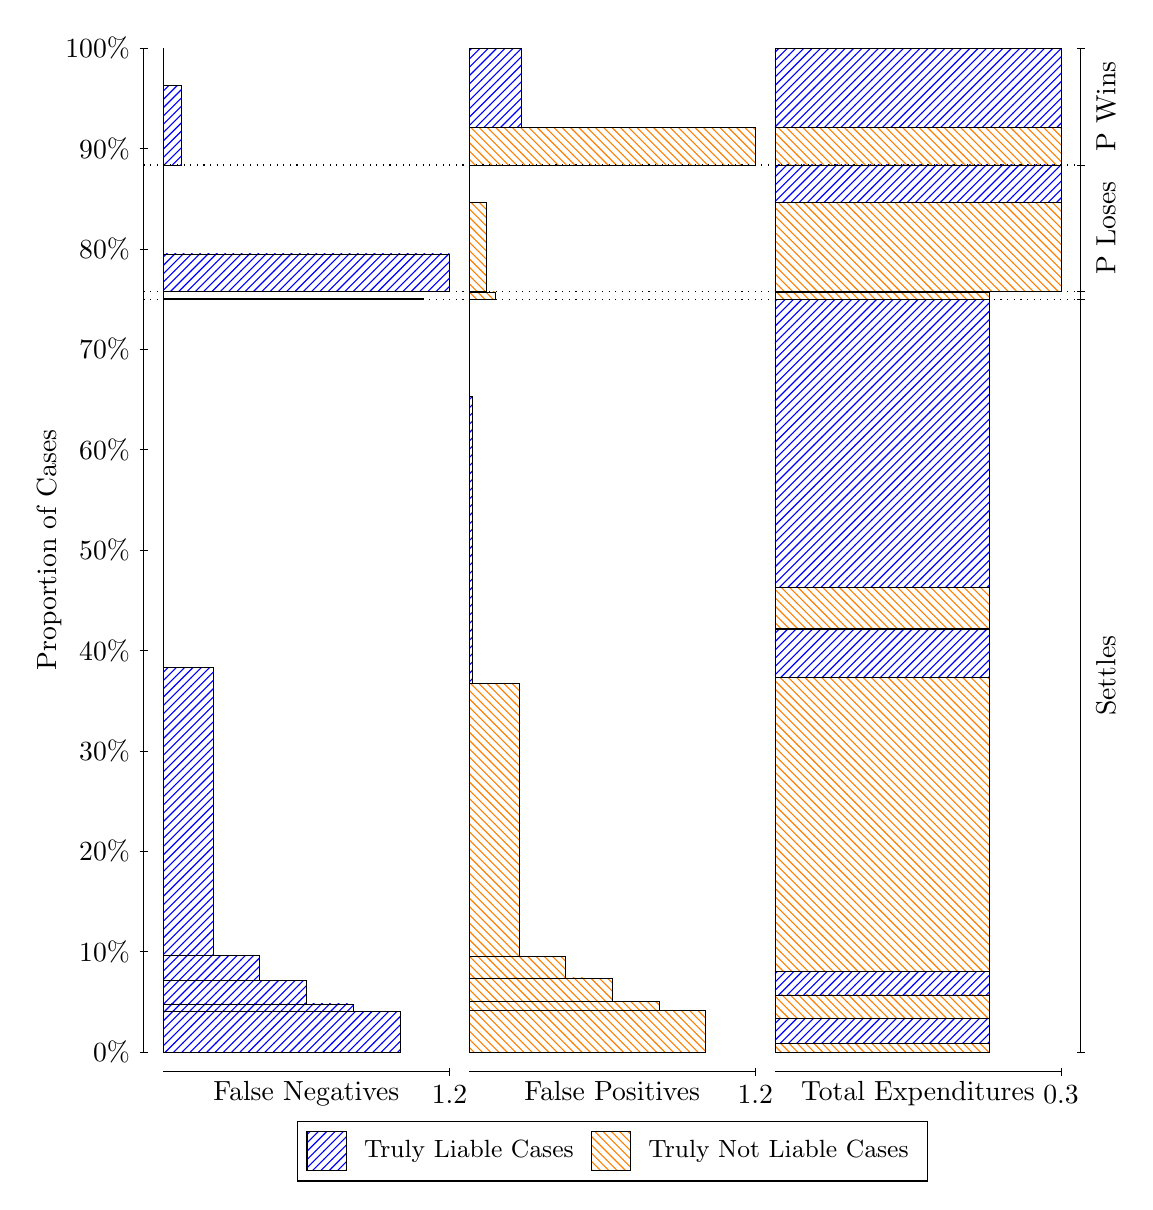
\begin{tikzpicture}
\draw[black, very thin] (1.5,1.75) -- (1.5,14.5);
\node[rotate=90, anchor=center] at (0.3, 8.125) {Proportion of Cases};
\draw[black, very thin] (1.45,1.75) -- (1.55,1.75);
\node[anchor=east] at (1.45, 1.75) {0\%};
\draw[black, very thin] (1.45,3.025) -- (1.55,3.025);
\node[anchor=east] at (1.45, 3.025) {10\%};
\draw[black, very thin] (1.45,4.3) -- (1.55,4.3);
\node[anchor=east] at (1.45, 4.3) {20\%};
\draw[black, very thin] (1.45,5.575) -- (1.55,5.575);
\node[anchor=east] at (1.45, 5.575) {30\%};
\draw[black, very thin] (1.45,6.85) -- (1.55,6.85);
\node[anchor=east] at (1.45, 6.85) {40\%};
\draw[black, very thin] (1.45,8.125) -- (1.55,8.125);
\node[anchor=east] at (1.45, 8.125) {50\%};
\draw[black, very thin] (1.45,9.4) -- (1.55,9.4);
\node[anchor=east] at (1.45, 9.4) {60\%};
\draw[black, very thin] (1.45,10.675) -- (1.55,10.675);
\node[anchor=east] at (1.45, 10.675) {70\%};
\draw[black, very thin] (1.45,11.95) -- (1.55,11.95);
\node[anchor=east] at (1.45, 11.95) {80\%};
\draw[black, very thin] (1.45,13.225) -- (1.55,13.225);
\node[anchor=east] at (1.45, 13.225) {90\%};
\draw[black, very thin] (1.45,14.5) -- (1.55,14.5);
\node[anchor=east] at (1.45, 14.5) {100\%};

\draw[black, very thin] (13.4,1.75) -- (13.4,14.5);
\draw[black, very thin] (13.35,1.75) -- (13.45,1.75);
\node[anchor=west] at (13.35, 1.75) {};
\draw[black, very thin] (13.35,11.308) -- (13.45,11.308);
\node[anchor=west] at (13.35, 11.308) {};
\draw[black, very thin] (13.35,11.413) -- (13.45,11.413);
\node[anchor=west] at (13.35, 11.413) {};
\draw[black, very thin] (13.35,13.015) -- (13.45,13.015);
\node[anchor=west] at (13.35, 13.015) {};
\draw[black, very thin] (13.35,14.5) -- (13.45,14.5);
\node[anchor=west] at (13.35, 14.5) {};

\draw[black, very thin, pattern color=blue, pattern=north east lines] (1.75,1.75) rectangle (4.7531,2.2657);
\draw[black, very thin, pattern color=blue, pattern=north east lines] (1.75,2.2657) rectangle (4.1599,2.3613);
\draw[black, very thin, pattern color=blue, pattern=north east lines] (1.75,2.3613) rectangle (3.8633,2.362);
\draw[black, very thin, pattern color=blue, pattern=north east lines] (1.75,2.362) rectangle (3.5667,2.6591);
\draw[black, very thin, pattern color=blue, pattern=north east lines] (1.75,2.6591) rectangle (3.2701,2.6601);
\draw[black, very thin, pattern color=blue, pattern=north east lines] (1.75,2.6601) rectangle (2.9735,2.9738);
\draw[black, very thin, pattern color=blue, pattern=north east lines] (1.75,2.9738) rectangle (2.6769,2.9749);
\draw[black, very thin, pattern color=blue, pattern=north east lines] (1.75,2.9749) rectangle (2.3803,6.6298);
\draw[black, very thin, pattern color=orange, pattern=north west lines] (1.75,6.6298) rectangle (1.75,11.308);
\draw[black, very thin, pattern color=blue, pattern=north east lines] (1.75,11.308) rectangle (5.0497,11.317);
\draw[black, very thin, pattern color=orange, pattern=north west lines] (1.75,11.317) rectangle (1.75,11.413);
\draw[black, very thin, pattern color=blue, pattern=north east lines] (1.75,11.413) rectangle (5.3833,11.886);
\draw[black, very thin, pattern color=orange, pattern=north west lines] (1.75,11.886) rectangle (1.75,13.015);
\draw[black, very thin, pattern color=blue, pattern=north east lines] (1.75,13.015) rectangle (1.9724,14.027);
\draw[black, very thin, pattern color=orange, pattern=north west lines] (1.75,14.027) rectangle (1.75,14.5);
\draw[black, very thin, pattern color=orange, pattern=north west lines] (5.6333,1.75) rectangle (8.6364,2.2777);
\draw[black, very thin, pattern color=orange, pattern=north west lines] (5.6333,2.2777) rectangle (8.3398,2.2798);
\draw[black, very thin, pattern color=orange, pattern=north west lines] (5.6333,2.2798) rectangle (8.0432,2.3915);
\draw[black, very thin, pattern color=orange, pattern=north west lines] (5.6333,2.3915) rectangle (7.7466,2.3934);
\draw[black, very thin, pattern color=orange, pattern=north west lines] (5.6333,2.3934) rectangle (7.45,2.6891);
\draw[black, very thin, pattern color=orange, pattern=north west lines] (5.6333,2.6891) rectangle (7.1534,2.6922);
\draw[black, very thin, pattern color=orange, pattern=north west lines] (5.6333,2.6922) rectangle (6.8568,2.9597);
\draw[black, very thin, pattern color=orange, pattern=north west lines] (5.6333,2.9597) rectangle (6.2636,6.4278);
\draw[black, very thin, pattern color=blue, pattern=north east lines] (5.6333,6.4278) rectangle (5.6704,10.083);
\draw[black, very thin, pattern color=blue, pattern=north east lines] (5.6333,10.083) rectangle (5.6333,11.308);
\draw[black, very thin, pattern color=orange, pattern=north west lines] (5.6333,11.308) rectangle (5.967,11.403);
\draw[black, very thin, pattern color=blue, pattern=north east lines] (5.6333,11.403) rectangle (5.6333,11.413);
\draw[black, very thin, pattern color=orange, pattern=north west lines] (5.6333,11.413) rectangle (5.8558,12.542);
\draw[black, very thin, pattern color=blue, pattern=north east lines] (5.6333,12.542) rectangle (5.6333,13.015);
\draw[black, very thin, pattern color=orange, pattern=north west lines] (5.6333,13.015) rectangle (9.2667,13.488);
\draw[black, very thin, pattern color=blue, pattern=north east lines] (5.6333,13.488) rectangle (6.3007,14.5);
\draw[black, very thin, pattern color=orange, pattern=north west lines] (9.5167,1.75) rectangle (12.242,1.8638);
\draw[black, very thin, pattern color=blue, pattern=north east lines] (9.5167,1.8638) rectangle (12.242,2.1786);
\draw[black, very thin, pattern color=orange, pattern=north west lines] (9.5167,2.1786) rectangle (12.242,2.4742);
\draw[black, very thin, pattern color=blue, pattern=north east lines] (9.5167,2.4742) rectangle (12.242,2.7713);
\draw[black, very thin, pattern color=orange, pattern=north west lines] (9.5167,2.7713) rectangle (12.242,6.5068);
\draw[black, very thin, pattern color=blue, pattern=north east lines] (9.5167,6.5068) rectangle (12.242,7.1182);
\draw[black, very thin, pattern color=orange, pattern=north west lines] (9.5167,7.1182) rectangle (12.242,7.1233);
\draw[black, very thin, pattern color=blue, pattern=north east lines] (9.5167,7.1233) rectangle (12.242,7.125);
\draw[black, very thin, pattern color=orange, pattern=north west lines] (9.5167,7.125) rectangle (12.242,7.6527);
\draw[black, very thin, pattern color=blue, pattern=north east lines] (9.5167,7.6527) rectangle (12.242,11.308);
\draw[black, very thin, pattern color=orange, pattern=north west lines] (9.5167,11.308) rectangle (12.242,11.403);
\draw[black, very thin, pattern color=blue, pattern=north east lines] (9.5167,11.403) rectangle (12.242,11.413);
\draw[black, very thin, pattern color=orange, pattern=north west lines] (9.5167,11.413) rectangle (13.15,12.542);
\draw[black, very thin, pattern color=blue, pattern=north east lines] (9.5167,12.542) rectangle (13.15,13.015);
\draw[black, very thin, pattern color=orange, pattern=north west lines] (9.5167,13.015) rectangle (13.15,13.488);
\draw[black, very thin, pattern color=blue, pattern=north east lines] (9.5167,13.488) rectangle (13.15,14.5);
\draw[black, dotted] (1.5,11.308) -- (13.4,11.308);
\draw[black, dotted] (1.5,11.413) -- (13.4,11.413);
\draw[black, dotted] (1.5,13.015) -- (13.4,13.015);
\draw[black, very thin] (1.75,1.5) -- (5.3833,1.5);
\node[anchor=north] at (3.5667, 1.5) {False Negatives};
\draw[black, very thin] (5.3833,1.45) -- (5.3833,1.55);
\node[anchor=north] at (5.3833, 1.45) {1.2};

\draw[black, very thin] (5.6333,1.5) -- (9.2667,1.5);
\node[anchor=north] at (7.45, 1.5) {False Positives};
\draw[black, very thin] (9.2667,1.45) -- (9.2667,1.55);
\node[anchor=north] at (9.2667, 1.45) {1.2};

\draw[black, very thin] (9.5167,1.5) -- (13.15,1.5);
\node[anchor=north] at (11.333, 1.5) {Total Expenditures};
\draw[black, very thin] (13.15,1.45) -- (13.15,1.55);
\node[anchor=north] at (13.15, 1.45) {0.3};

\node[black, centered, rotate=90] at (13.72, 6.5288) {Settles};

\node[black, centered, rotate=90] at (13.72, 12.214) {P Loses};
\node[black, centered, rotate=90] at (13.72, 13.758) {P Wins};

\draw (7.449999999999999,1.5) node[draw=none] (baseCoordinate) {};
\begin{scope}[align=center]
        \matrix[scale=0.5, draw=black, below=0.5cm of baseCoordinate, nodes={draw}, column sep=0.1cm]{
            \node[rectangle, draw, minimum width=0.5cm, minimum height=0.5cm, pattern=north east lines, pattern color=blue] {}; &
            \node[draw=none, font=\small] (B) {Truly Liable Cases}; &
            \node[rectangle, draw, minimum width=0.5cm, minimum height=0.5cm, pattern=north west lines, pattern color=orange] {}; &
            \node[draw=none, font=\small] (B) {Truly Not Liable Cases}; \\
            };
\end{scope}

\end{tikzpicture}
\end{document}